\subsection{Caso d'uso UC4: Visualizzazione}
\begin{figure}[h] 
	\centering 
	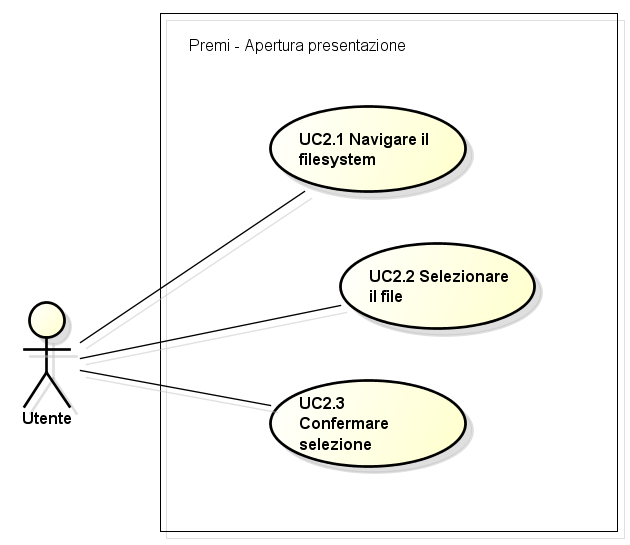
\includegraphics[scale=0.45] {img/UC4.png}
	\caption{UC4 - Visualizzazione} 
\end{figure}

\begin{itemize}
	\item \textbf{Attori:} Utente non autenticato, utente autenticato;
	\item \textbf{Scopo e descrizione:} Un utente, una volta aperto un progetto, può scegliere se visualizzare una presentazione o un'\gls{infografica};
	\item \textbf{Precondizione:} Il sistema mostra all'utente un progetto;
	\item \textbf{Flusso principale degli eventi:}
	\begin{enumerate}
		\item L'utente sceglie di visualizzare una presentazione [UC4.1];
		\item L'utente sceglie di visualizzare un'\gls{infografica} [UC4.2].
	\end{enumerate}
	\item \textbf{Postcondizione:} Il sistema mostra all'utente la schermata di visualizzazione di una presentazione o di un'\gls{infografica} a seconda di cosa è stato scelto.
\end{itemize}

\subsection{Caso d'uso UC4.1: Visualizzazione di una presentazione}
\begin{figure}[h] 
	\centering 
	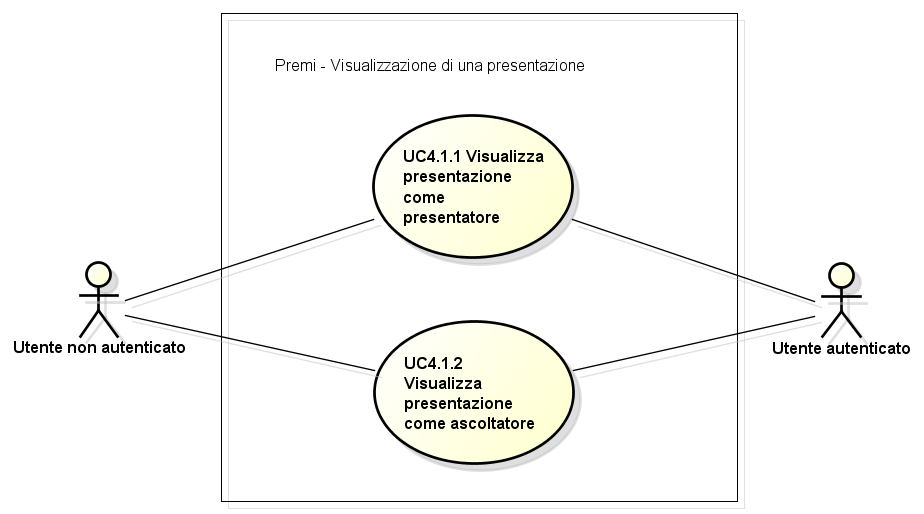
\includegraphics[scale=0.45] {img/UC4.1.png}
	\caption{UC4.1 - Visualizzazione di una presentazione} 
\end{figure}

\begin{itemize}
	\item \textbf{Attori:} Utente non autenticato, utente autenticato;
	\item \textbf{Scopo e descrizione:} La visualizzazione di una presentazione permette di scorrere le \gls{slide}. In generale, la presentazione segue un flusso principale, da sinistra a destra, e un flusso secondario, dall'alto verso il basso.\\
	Durante il passaggio da una \gls{slide} all'altra nel flusso principale avverrà un effetto di "zoom-out, zoom-in" con il quale è possibile avere una panoramica della presentazione e soprattutto delle \gls{slide} successive.\\
	L'utente può scegliere se visualizzare la presentazione come presentatore o come ascoltatore;
	\item \textbf{Precondizione:} L'utente ha scelto di visualizzare una presentazione esistente;
	\item \textbf{Flusso principale degli eventi:}
	\begin{enumerate}
		\item L'utente sceglie di visualizzare la presentazione come presentatore [UC4.1.1];
		\item L'utente sceglie di visualizzare la presentazione come ascoltatore [UC4.1.2];
		\item L'utente si sposta tra le \gls{slide} [UC4.1.3];
	\end{enumerate}
	\item \textbf{Postcondizione:} Il sistema mostra all'utente la schermata di visualizzazione di una presentazione con le impostazioni scelte.
\end{itemize}

\subsection{Caso d'uso UC4.1.1: Visualizzare una presentazione come presentatore}
\begin{itemize}
	\item \textbf{Attori:} Utente non autenticato, utente autenticato;
	\item \textbf{Scopo e descrizione:} L'utente ha scelto di visualizzare la presentazione come presentatore e il sistema mostra la presentazione con il supporto visivo dedicato al presentatore;
	\item \textbf{Precondizione:} L'utente ha scelto di visualizzare la presentazione come presentatore;
	\item \textbf{Postcondizione:} Il sistema avvia la presentazione con il supporto visivo dedicato al presentatore.
\end{itemize}

\subsection{Caso d'uso UC4.1.2: Visualizzare una presentazione come ascoltatore}
\begin{itemize}
	\item \textbf{Attori:} Utente non autenticato, utente autenticato;
	\item \textbf{Scopo e descrizione:} L'utente ha scelto di visualizzare la presentazione come ascoltatore e il sistema mostra la presentazione selezionata;
	\item \textbf{Precondizione:} L'utente ha scelto di visualizzare la presentazione come ascoltatore;
	\item \textbf{Postcondizione:} Il sistema avvia la presentazione.
\end{itemize}

\subsection{Caso d'uso UC4.1.3: Spostarsi tra le slide}
\begin{itemize}
	\item \textbf{Attori:} Utente non autenticato, utente autenticato;
	\item \textbf{Scopo e descrizione:} L'utente sta visualizzando una presentazione e vuole cambiare \gls{slide}. Si può muovere nella quattro direzioni così da procedere sia nel flusso principale che in quello secondario;
	\item \textbf{Precondizione:} L'utente sta visualizzando la presentazione;
	\item \textbf{Postcondizione:} Il sistema ha cambiando la \gls{slide} a seconda del comando dato dall'utente.
\end{itemize}


\subsection{Caso d'uso UC4.2: Visualizzazione di un'infografica}
\begin{itemize}
	\item \textbf{Attori:} Utente non autenticato, utente autenticato;
	\item \textbf{Scopo e descrizione:} L'utente ha scelto di visualizzare un'\gls{infografica} e il sistema la mostra;
	\item \textbf{Precondizione:} L'utente ha scelto di visualizzare un'\gls{infografica};
	\item \textbf{Postcondizione:} Il sistema mostra all'utente la schermata di visualizzazione dell'\gls{infografica}.
\end{itemize}

